%%%%%%%%%%%%%%%%%%%%%%%%%%%%%%%%%%%%%%%%%
% baposter Portrait Poster
% LaTeX Template
% Version 1.0 (15/5/13)
%
% Created by:
% Brian Amberg (baposter@brian-amberg.de)
%
% This template has been downloaded from:
% http://www.LaTeXTemplates.com
%
% License:
% CC BY-NC-SA 3.0 (http://creativecommons.org/licenses/by-nc-sa/3.0/)
%
%%%%%%%%%%%%%%%%%%%%%%%%%%%%%%%%%%%%%%%%%

%----------------------------------------------------------------------------------------
%	PACKAGES AND OTHER DOCUMENT CONFIGURATIONS
%----------------------------------------------------------------------------------------

\documentclass[a0paper,portrait]{baposter}

\usepackage[font=small,labelfont=bf]{caption} % Required for specifying captions to tables and figures
\usepackage{booktabs} % Horizontal rules in tables
\usepackage{relsize} % Used for making text smaller in some places
\usepackage{multicol} % This is so we can have multiple columns of text side-by-side
\columnsep=100pt % This is the amount of white space between the columns in the poster
\columnseprule=3pt % This is the thickness of the black line between the columns in the poster

\usepackage{times} % Use the times font
%\usepackage{palatino} % Uncomment to use the Palatino font
\usepackage[ngerman]{babel}
\usepackage[utf8]{inputenc}
\usepackage{graphicx} % Required for including images
\usepackage{float}
\usepackage{subcaption}
\usepackage{sidecap}
\usepackage{enumitem} %für Nummerierung
\graphicspath{{figures/}} % Location of the graphics files
\usepackage{booktabs} % Top and bottom rules for table
\usepackage[font=small,labelfont=bf]{caption} % Required for specifying captions to tables and figures
\usepackage{amsfonts, amsmath, amsthm, amssymb} % For math fonts, symbols and environments
\usepackage{wrapfig} % Allows wrapping text around tables and figures

\graphicspath{{figures/}} % Directory in which figures are stored

\definecolor{bordercol}{RGB}{40,40,40} % Border color of content boxes
\definecolor{headercol1}{RGB}{186,215,230} % Background color for the header in the content boxes (left side)
\definecolor{headercol2}{RGB}{80,80,80} % Background color for the header in the content boxes (right side)
\definecolor{headerfontcol}{RGB}{0,0,0} % Text color for the header text in the content boxes
\definecolor{boxcolor}{RGB}{186,215,230} % Background color for the content in the content boxes

\begin{document}

\background{ % Set the background to an image (background.pdf)
\begin{tikzpicture}[remember picture,overlay]
\draw (current page.north west)+(-2em,2em) node[anchor=north west]
{\includegraphics[height=1.1\textheight]{background}};
\end{tikzpicture}
}

\begin{poster}{
grid=false,
borderColor=bordercol, % Border color of content boxes
headerColorOne=headercol1, % Background color for the header in the content boxes (left side)
headerColorTwo=headercol2, % Background color for the header in the content boxes (right side)
headerFontColor=headerfontcol, % Text color for the header text in the content boxes
boxColorOne=boxcolor, % Background color for the content in the content boxes
headershape=roundedright, % Specify the rounded corner in the content box headers
headerfont=\Large\sf\bf, % Font modifiers for the text in the content box headers
textborder=rectangle,
background=user,
headerborder=open, % Change to closed for a line under the content box headers
boxshade=plain
}
{}
%
%----------------------------------------------------------------------------------------
%	TITLE AND AUTHOR NAME
%----------------------------------------------------------------------------------------
%
{\sf\bf Nichtlineare Optik} % Poster title
{\vspace{1em} von Juliane Ratzsch \& Gentian Rrafshi} % Author email addresses
{
\includegraphics[scale=1]{logo}} % University/lab logo

%\veryHuge \color{NavyBlue} \textbf{Nichtlineare Optik} \color{Black}\\ % Title
%\huge \textbf{Juliane Ratzsch \& Gentian Rrafshi} % Author(s)
%\end{minipage}
%%
%\begin{minipage}[b]{0.25\linewidth}
%
\includegraphics[width=20cm]{logo.png}
%\end{minipage}

%----------------------------------------------------------------------------------------
%	INTRODUCTION
%----------------------------------------------------------------------------------------

\headerbox{Ziel des Versuchs}{name=introduction,column=0,row=0}{


An einem Nd:YAG-Laser wird untersucht:
\begin{enumerate}
\item[-] die Ausgangsleistung als Funktion verschiedener Parameter
\item[-] Frequenzverdopplung
\item[-] Pulsbetrieb mit Güteschaltung
\end{enumerate}
}

%----------------------------------------------------------------------------------------
%	MATERIALS AND METHODS
%----------------------------------------------------------------------------------------

\headerbox{Grundlagen}{name=methods,column=0,below=introduction}{


%\begin{figure}[H]
%\centering
%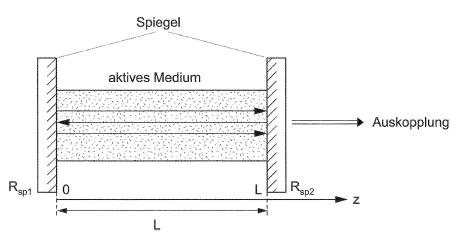
\includegraphics[scale=0.25]{schematischerAufbau} 
%\caption{Aufbauschema}
%\end{figure}
Ein Laser besteht aus einer Energiepumpe, einem aktivem Medium und einem optischen Resonator. \par
In diesem Versuch behandeln wir ein Vier-Niveau-System-Laser. 
Das Termschema hierfür:
\begin{figure}[H]
\centering
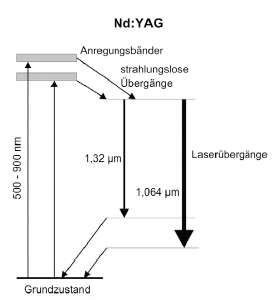
\includegraphics[scale=0.5]{Term}
\caption{Termschema Nd:YAG-Laser}
\end{figure}
Die Polarisation im aktiven Medium wird beschrieben durch:
\begin{align*}
\textbf{P} = \epsilon_0\cdot\sum\limits_{n\in\mathbb{N}_0} \chi^{(n)}\textbf{E}^n.
\end{align*}
Die Entwicklungskoeffizienten sind ab der 2. Ordnung sehr klein.
Für große Intensitäten sind diese Terme aber relevant. Aus dem quadratischen Term ergibt sich die Frequenzverdopplung.

Um die Sekundärstrahlung abzustrahlen, muss eine Phasenanpassung durchgeführt werden
\begin{align*}
n(\omega) = n(2\cdot\omega).
\end{align*}
z.B. mit einem doppelbrechenden Kristall

\begin{figure}[H]
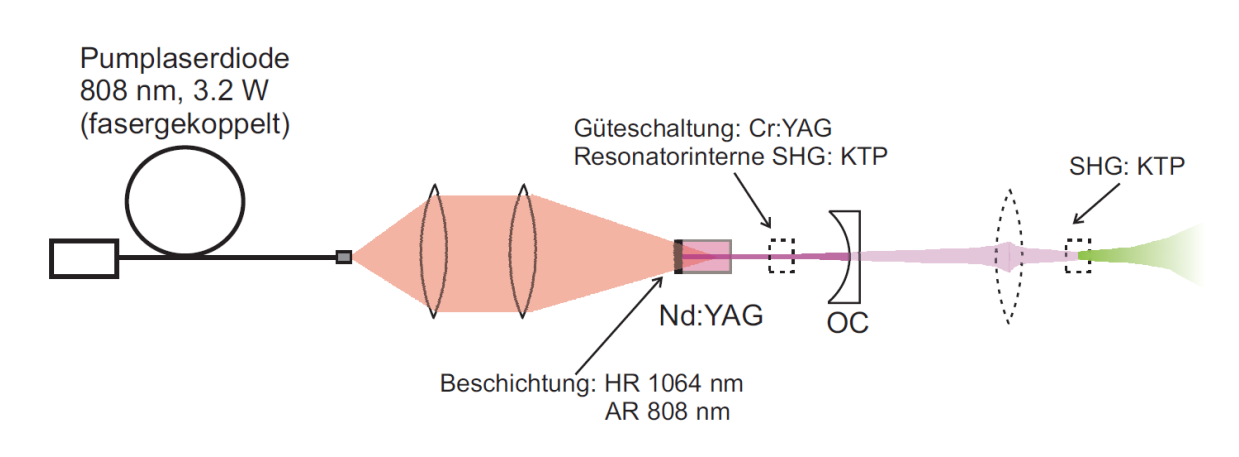
\includegraphics[scale=0.3]{frequenzverdoppelung} 
\caption{schemetische Darstellung der Frequenzverdopplung}
\end{figure}
}

%----------------------------------------------------------------------------------------
%	CONCLUSION
%----------------------------------------------------------------------------------------

\headerbox{Zusammenfassung}{name=conclusion,column=0,below=methods}{

\begin{enumerate}[itemsep=0pt] 
\item Die Pumpratenschwelle (1,8\,A) muss überschritten werden. Darüber steigt die Ausgangsleistung linear an. Das frequenzverdoppelte Licht hat eine geringe Ausgangsleistung.

\item Die Ausgangsleistung hängt stark vom Auskoppelungsgrad des Resonators ab.

\item Die theoretische Stabilitätsbedingung wurde experimentell bestätigt.

\item Im Pulsbetrieb steigt die Repetitionsrate mit dem Diodenstrom.
\end{enumerate}
}

%----------------------------------------------------------------------------------------
%	RESULTS 1
%----------------------------------------------------------------------------------------

\headerbox{Auswertung}{name=results1,span=2,column=1,row=0}{ % To reduce this block to 1 column width, remove 'span=2'
\subsection*{Ausgangsleistung als Funktion des Diodenstroms}
\begin{figure}[H]
\centering
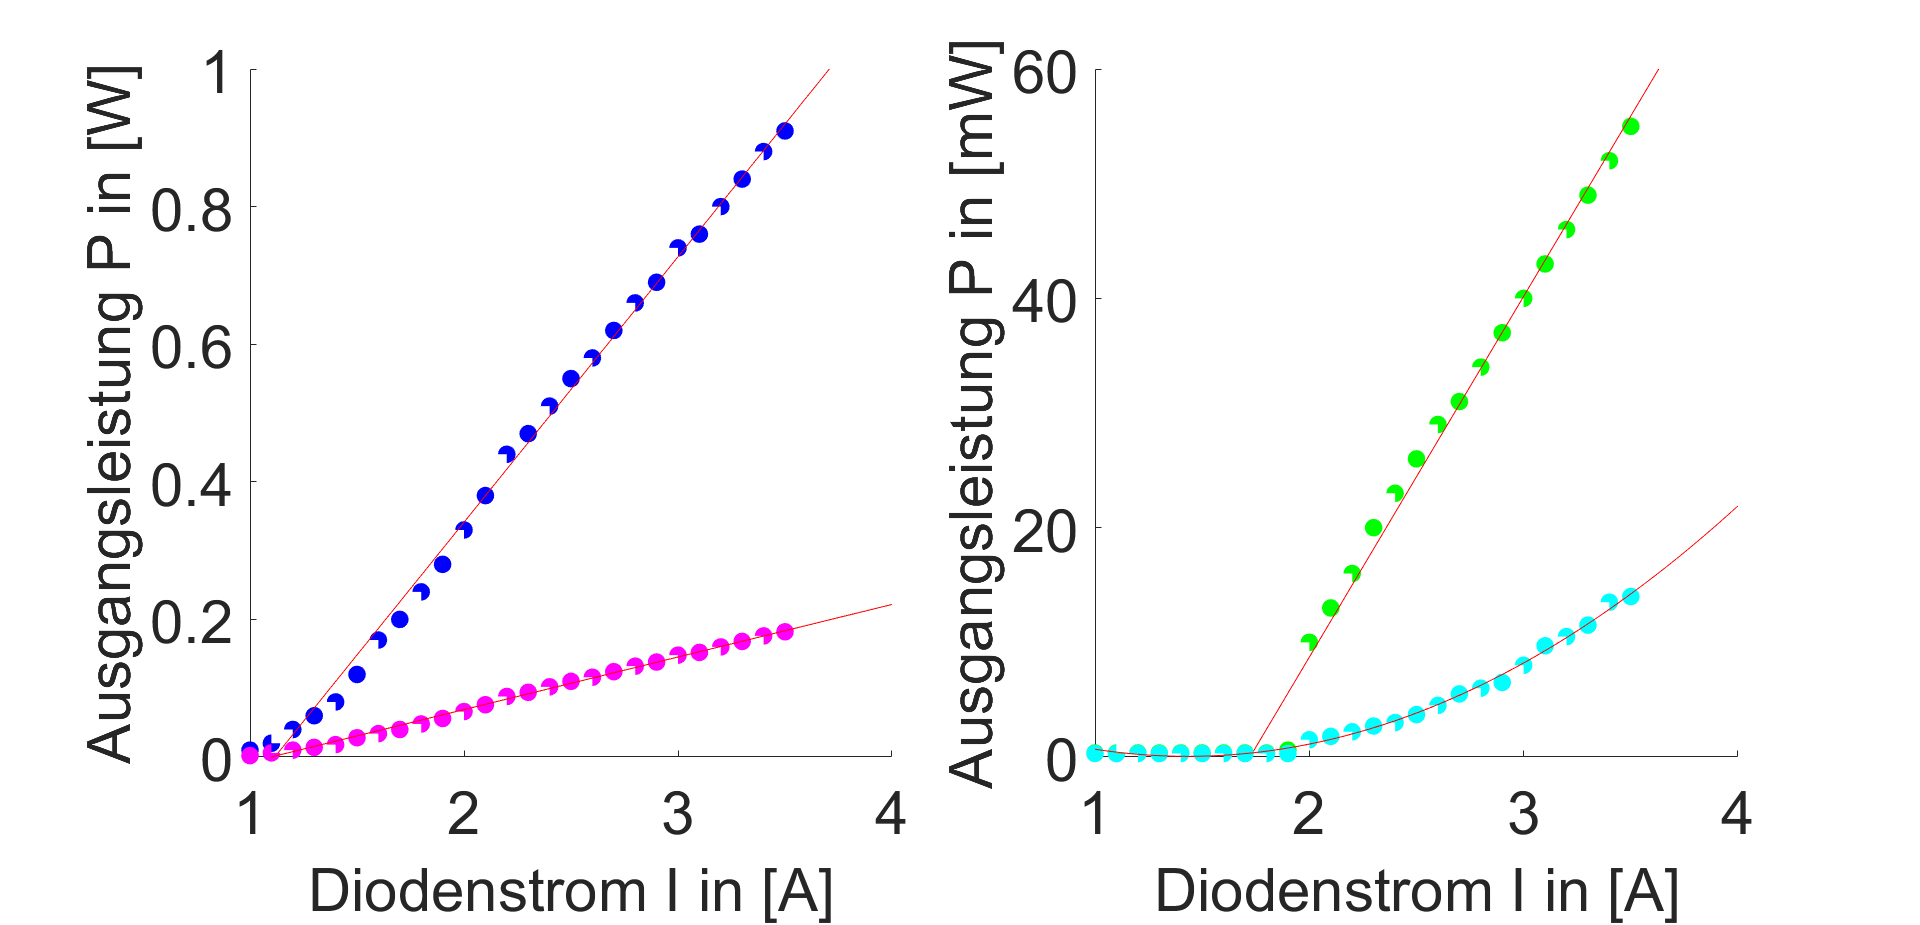
\includegraphics[scale=0.17]{Diodenstrom} 
\caption{Ausgangsleistung als Funktion des Diodenstroms für den cw- Laser (blau), den gepulsten Laser (magenta), für die resonatorexterne Frequenzverdopplung (grün) und für die resonatorinterne Frequenzverdopplung (Cyan).}
%am besten spezifikation in der legende
\end{figure}
Außer bei der resonatorinternen Frequenzverdopplung ist der Anstieg der Ausgangsleistung linear. Bei der resonatorinternen Frequenzverdopplung quadratisch.

\subsection*{Die Ausgangsleistung bei verschiedenen Auskoppelungsgraden}
% das war ihm auch zu ausführlich, wenn ich mich richtig erinnere?
\begin{figure}[H]
\centering
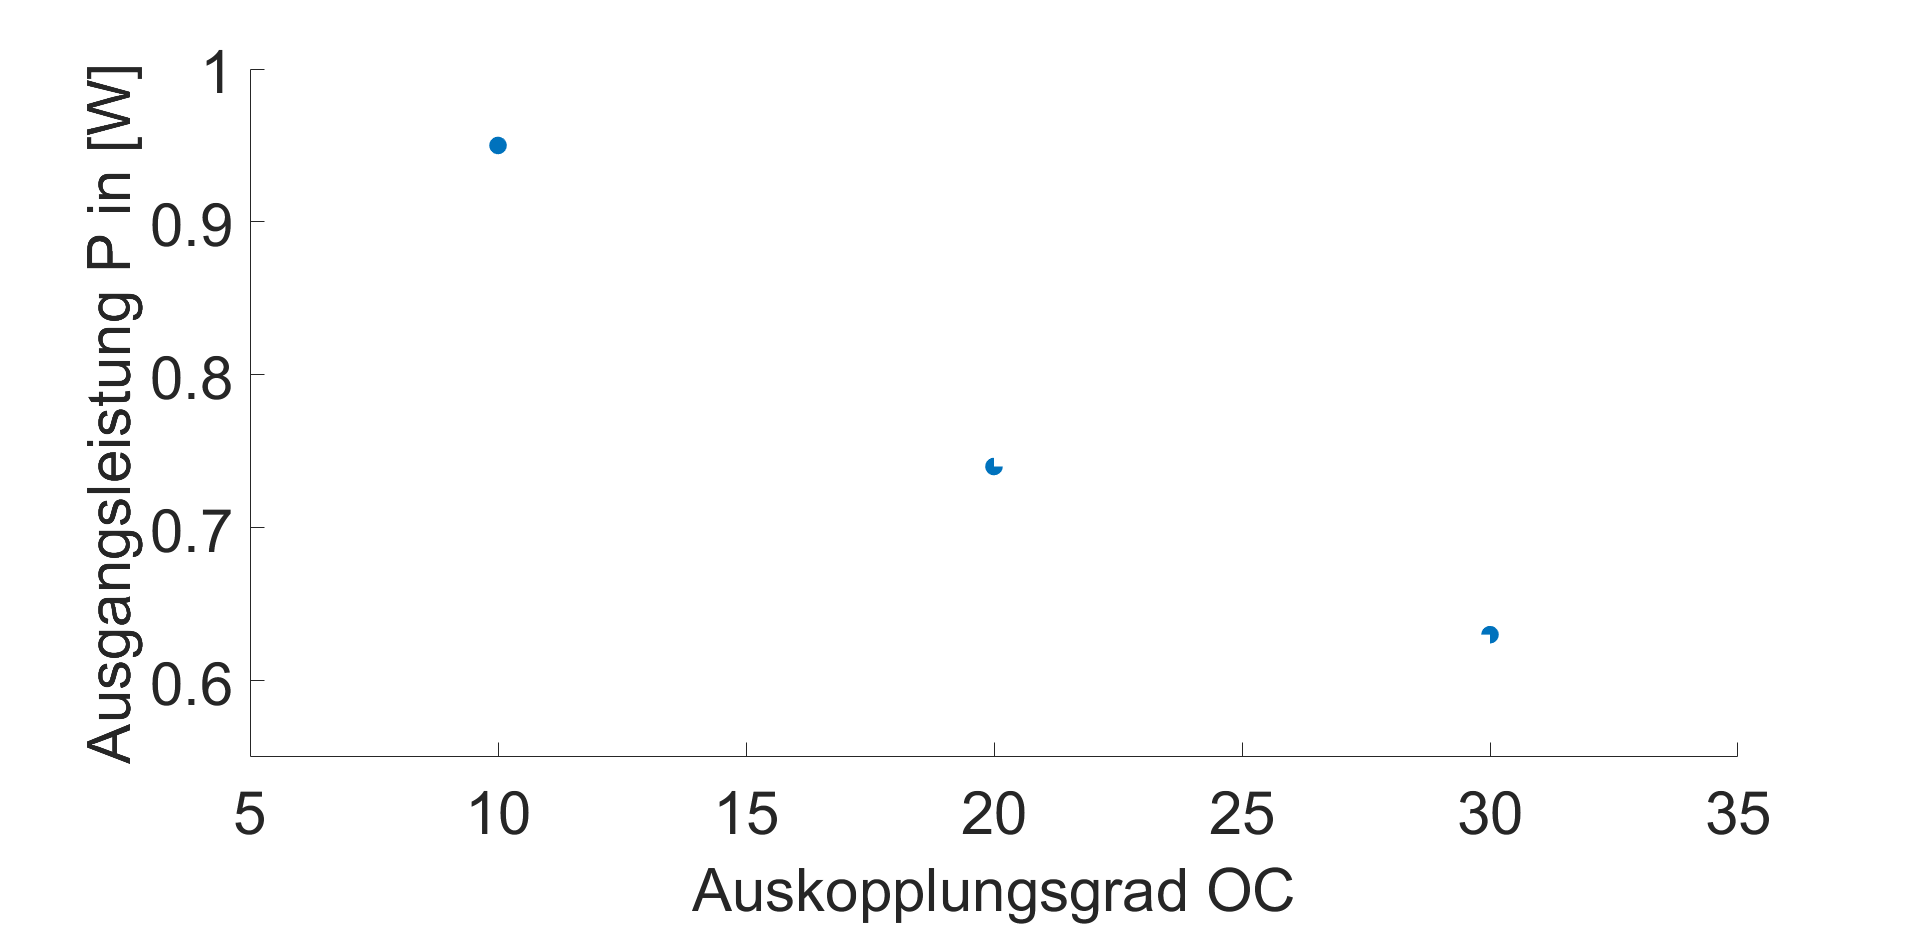
\includegraphics[scale=0.17]{Auskopplungsgrad} 
\caption{Die Ausgangsleistung bei verschiedenen Auskoppelungsgraden}
\end{figure}
Die beste Leistung wird bei einem Auskopplungsgrad von 10\% erreicht. Das stimmt mit der Theorie überein:
\begin{align*}
\text{P(OC)}=-\frac{\text{E}_{\text{sat}} \cdot \text{OC}}{\tau_{\text{L}}}\cdot \left[  \frac{2 \text{g}_0}{\text{ln}\,(1-\text{OC})+ \text{ln}\,(1-s) }+ 1 \right] 
\end{align*}
Für $s\in\lbrace0.01,0.02\rbrace$ ist das optimale $\text{OC}_{\text{max}} \approx 0.11$, was einem Auskopplungsgrad von 11\% entspricht. 

\subsection*{Die Ausgangsleistung als Funktion der Resonatorlänge}
\begin{minipage}{0.5\textwidth}
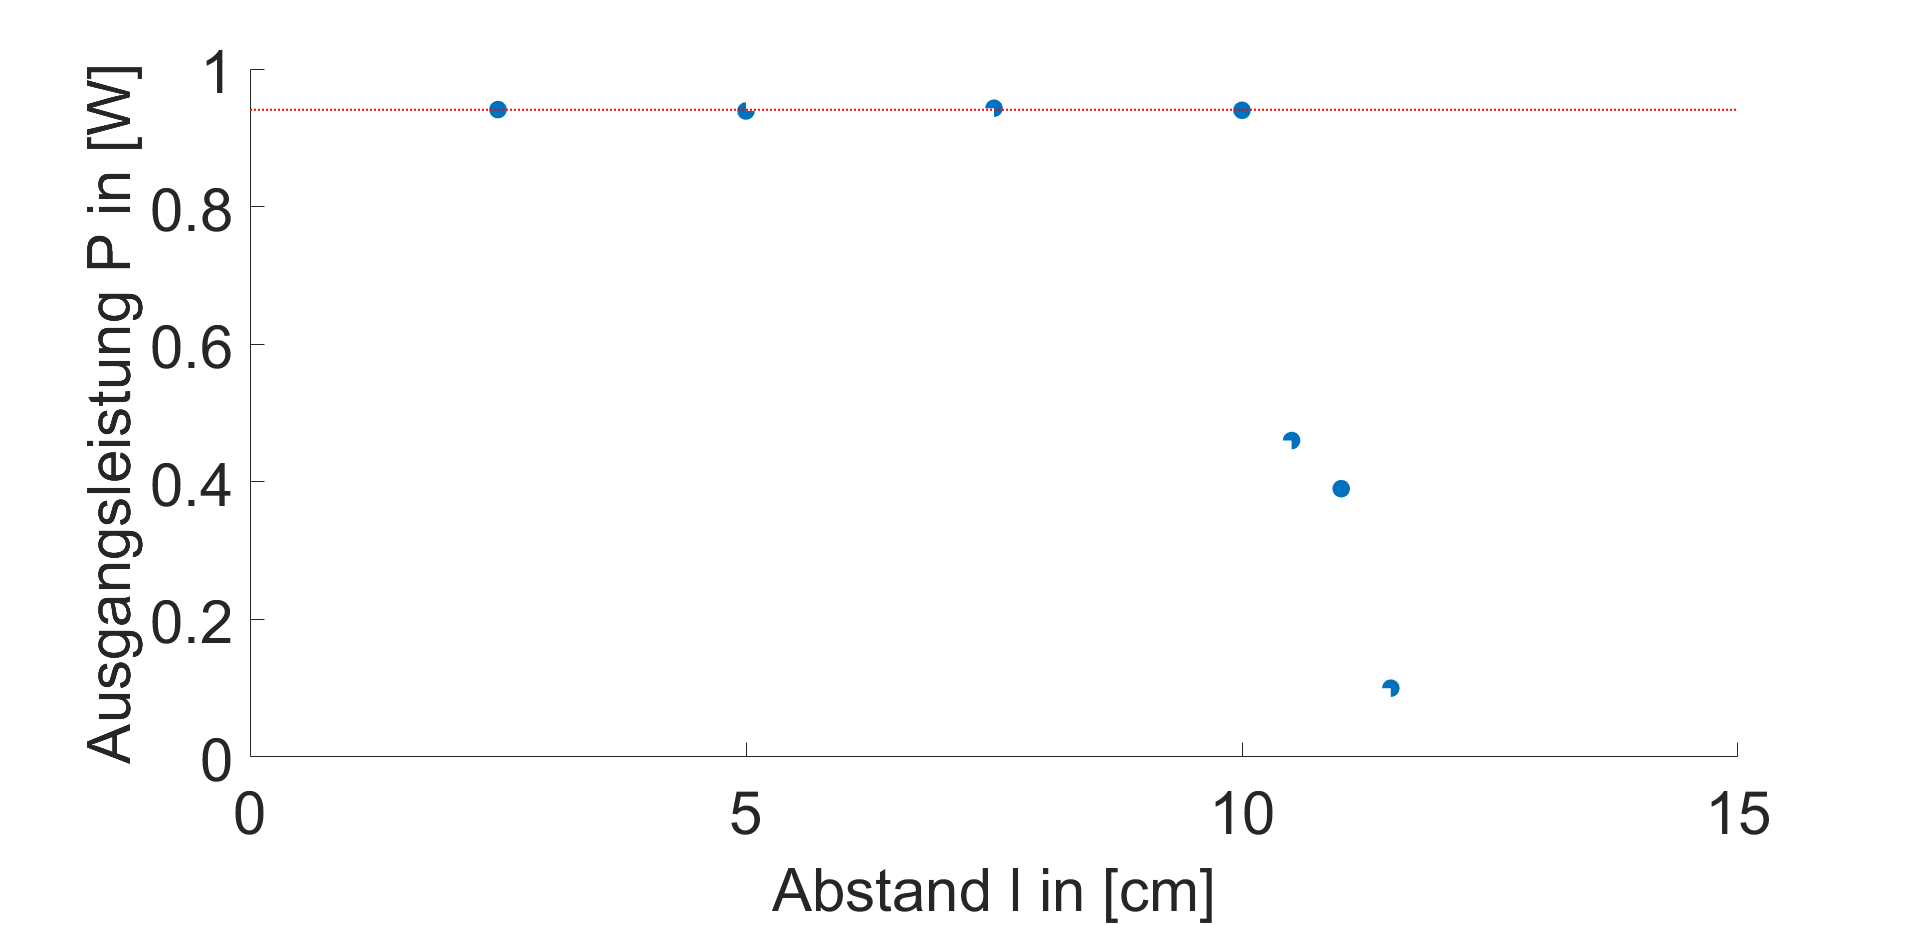
\includegraphics[scale=0.15]{Abstand} 
%\caption{Die Ausgangsleistung bei verschiedenen Resonatorlängen}
\end{minipage}
\begin{minipage}{0.5\textwidth}
Das Stabilitätskriterium, mit den Spiegelparametern $R_1=\infty$ und $R_2=100\,\text{mm}$ lautet:
\begin{align*}
0\leq \left(1-\frac{l}{100\,\text{mm}}\right)\leq 1.
\end{align*}
Für stabilen Betrieb muss die Resonatorlänge $
l\in\left[0\,\text{cm},10\,\text{cm}\right]$ sein. Die Messung bestätigt das. 
\end{minipage}
\subsection*{Die Repetitionsrate der Laserpulse in Abhängigkeit
vom Diodenstrom}
\begin{figure}[H]
\centering
\begin{subfigure}{0.45\textwidth}
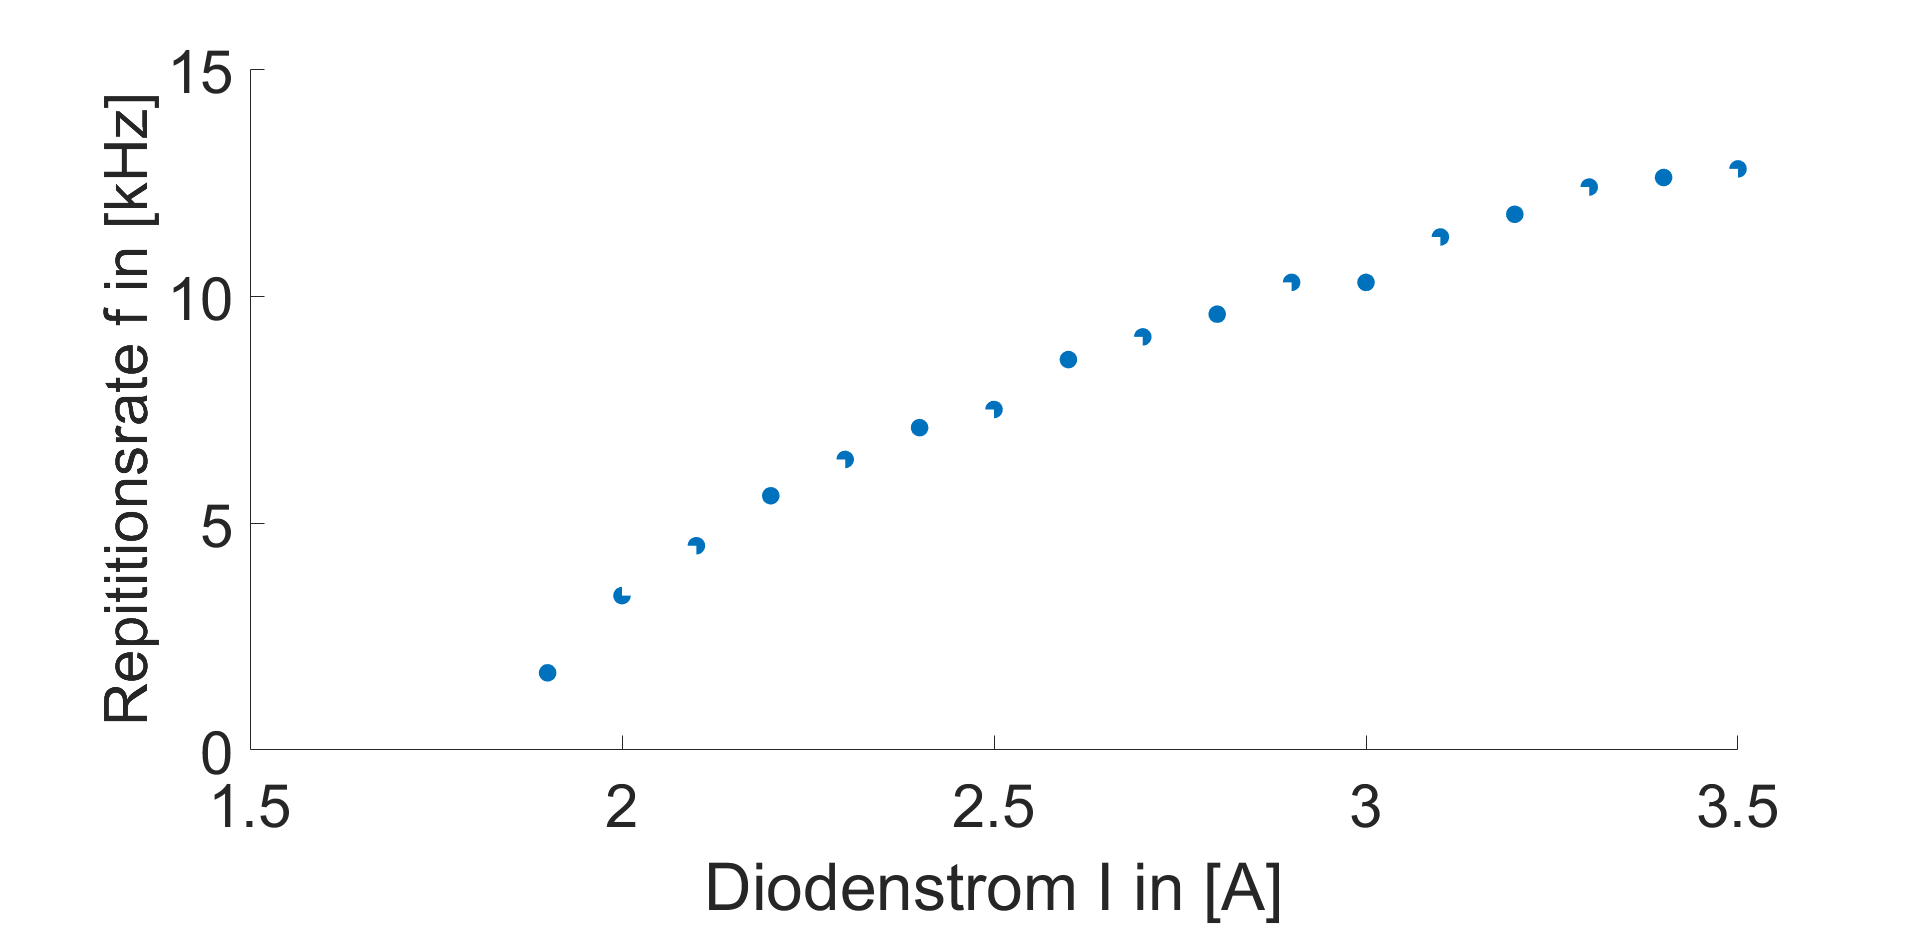
\includegraphics[scale=0.13]{frequenz} 
\caption{Repetitionsrate der Laserpulse in Abhängigkeit
vom Diodenstrom}
\label{bla}
\end{subfigure} %
\begin{subfigure}{0.45\textwidth}
\centering
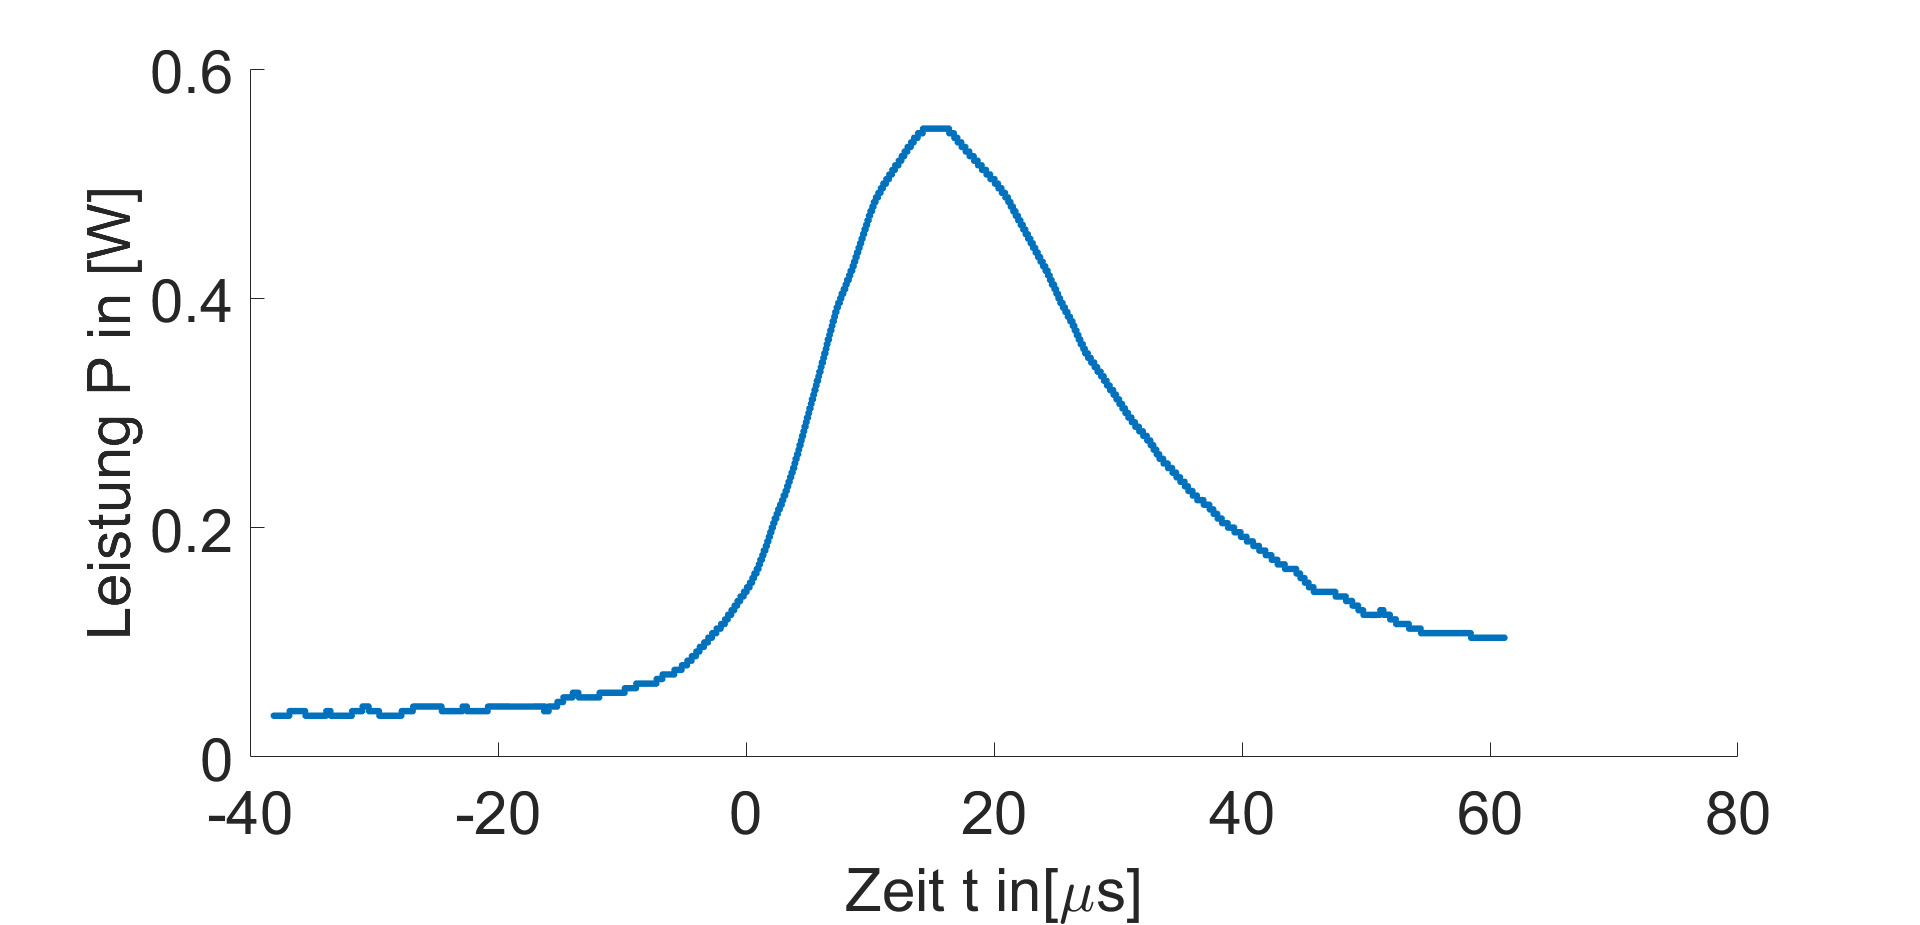
\includegraphics[scale=0.13]{Einzelpuls} 
\caption{Ein einzelner Laserpuls. Die Leistung eines gütegeschaltenen Lasers über die Zeit. }
\end{subfigure}
\end{figure}

Die Repetitionsrate liegt im kHz-Bereich liegt. 
Sie steigt mit steigendem Diodenstrom näherungsweise linear an, da bei größerer Pumpleistung die zur Besetzungsinversion benötigte Zeit sinkt.
Die Repetitionsrate strebt außerdem gegen eine maximale Frequenz, da der Q-Switch nicht beliebig schnell schalten kann.

}

%----------------------------------------------------------------------------------------

\end{poster}

\end{document}